\chapter{FITTING THE LOW RESOLUTION SPECTRUM OF \mrvel\ USING CONTINUUM MODELS} \label{chap:continuum}
    %\doublespacing
    \minitoc
    \emph{Abstract of chapter \ref{chap:continuum}}
    
    \section{The Luminous SSS \mrvel} \label{continuum:on-mrvel}
		The particular luminous galactic SSS known as MR Vel, and referred to as \mrvel, was discovered by Motch \emph{et al.} \cite{motch1994} in the ROSAT Galactic Plane Survey (RGPS), which is defined as the $|b|\le 20^{\circ}$ region of the ROSAT All Sky Survey. In the J2000 frame, the right ascension of the said source is 141.44042 and the declination is -47.96972 (RA=09 25 46.00; Dec=-47 58 17.4: as resolved by Simbad).
		
		\mrvel~ was the brightest SSS candidate source in RGPS, with ROSAT PSPC hardness ratios of $HR1=0.96\pm 0.03$ and $HR2=-0.69\pm 0.03$. Fitting a blackbody to the ROSAT observations, a hydrogen column density in the range $n_H=(1.4-3.7)\times 10^{22}\,\mathrm{cm}^{-2}$ can be obtained \cite{motch1994}. There is a considerable amount of uncertainty in current literature about its distance, with estimates ranging from  1 kpc to 10 kpc. Consulting the Data Release 2 from Gaia, one can find negligible parallax. This fact along with its high luminosity suggests that its distance is likely to be $>5$ kpc.
		
		Hartmann \emph{et al.} applied non-local thermodynamic equilibrium (NLTE) models, which included metal line opacities, to the spectrum extracted from the observations by BeppoSAX LECS of \mrvel~on January 25-26 1997 \cite{hartmann99}. They found that if a single model component is assumed for \mrvel, a large discrepancy is observed between the model and data above 1.19 keV. The emission above $\sim$ 1.2 kev (i.e. NeIX edge) can be accounted for by adding another spectral model component, viz. collisional ionization equilibrium.
		
		Higher resolution spectra obtained using grating spectroscopy by Chandra and XMM-Newton revealed complex structures in the spectra of \mrvel. Such spectra show the presence of P Cygni profiles of FeXVII and OVIII, which typically arise in a wind. Two groups, namely Bearda \emph{et al.} and Motch \emph{et al.} (2002) have come to the conclusion that the \mrvel~spectra, as observed by the Chandra HETGS and the XMM-Newton RGS, cannot be reproduced by LTE or NLTE model atmospheres \cite{bearda2002,motch2002}, even though there is little clarity on the reason for this. Obtaining an acceptable fit for \mrvel~spectrum assumes crucial importance at this juncture. It has been pointed out that in the absence of a proper model describing the emission spectrum, it becomes impossible to derive fundamental parameters such as temperature, density, gravity and luminosity \cite{motch2002}.
		
		\section{Journal of Observations} \label{continuum:obs}
			The plan to develop a robust model is two-fold:
			\begin{enumerate}
				\item Obtain a continuum model which includes interstellar absorption as well as absorption edges due to bound-free transitions, if necessary. \label{mod-step:01}
				\item Compute a synthetic spectrum that accounts for all the emission lines, and then superimpose this over the existing continuum model. \label{mod-step:02}
			\end{enumerate}
			
			Step \ref{mod-step:01} would require the use of the software package named Xspec \cite{xspecManualv12_9_1}, whereas step \ref{mod-step:02} would mainly require the use of the Tlusty and Synspec codes \cite{tlustymanualI}.

			Based on a private communication with Prof. Phil Charles from the University of Southampton, we took a cue using a reference to Ebisawa \emph{et al.}, who had to use an extra hard component or play with the O and Ne abundances massively to get a good fit \cite{ebisawa1996}. We have used the same ASCA observation to obtain the continuum model. Then we used that model on the EPIC-PN data from the \emph{same observation} for which we later tried to fit the RGS data from XMM-Newton for \mrvel. Given below are the three main observations that were considered.
			
			\subsection{By ASCA SIS1} \label{continuum:obs:asca}
				\mrvel~was observed for 20 ks with ASCA from 13:28 UT on 22-12-1994 to 02:02 UT on 23-12-1994 with the Solid State Spectrometer (SIS0 and SIS1) and the Gas Imaging Spectrometer (GIS2 and GIS3), each combined with an X-ray telescope \cite{ebisawa1996}. In this work, only the spectrum obtained from the SIS1 detector was analyzed.
				
			\subsection{By XMM-Newton EPIC-pn} \label{continuum:obs:xmm}
				\mrvel~was observed for 61.2 ks with XMM-Newton from 16-12-2000 to 17-12-2000 with the Optical Monitor (OM), European Photon Imaging Camera (EPIC MOS1, MOS2 and PN) and the Reflection Grating Spectrometer (RGS1 and RGS), the EPIC and RGS systems combined with 3 Wolter Type 1 optical systems \cite{motch2002}. This chapter discusses the fitting of the spectra obtained from the EPIC-PN detector. The analysis of the high resolution spectra obtained from the RGS detectors are discussed in chapter \ref{chap:hi-resolution}
		
		\section{Fitting of ASCA SIS1 Data} \label{continuum:asca}
			In their spectral analysis of \mrvel, Ebisawa \emph{et al.} fitted the observed spectrum -- first with a simple absorbed blackbody model and then with one comprising of and absorbed blackbody along with three absorption edges. We have first reproduced some of their results and them attempted to obtain a better fit because at present more accurate models are already available in Xspec.
			
			\subsection{Fitting using an Absorbed Blackbody} \label{continuum:asca:abs-bb}
				Ebisawa \emph{et al.} had used the ISM absorption model by Morrison \& McCammon \cite{morrison1983wabs}. This is implemented in Xspec by the multiplicative models named \texttt{Wabs} and \texttt{ZWabs}. We have fitted the same observation with a composite Xspec model -- \texttt{wabs*bbody}.
				
				However, this model neglects the contributions from ions, molecules, grains and abundance enhancements. An improvement, in this regard, is the Xspec model \texttt{ISMabs} \cite{ismabs_gatuzz}. So we then fitted the observations with another Xspec model -- \texttt{ismabs*bbody}.
				
				Figure \ref{asca:01} shows the spectrum fitted using a simple absorbed blackbody model, with \texttt{Wabs} used to approximate the interstellar absorption. On the other hand, figure \ref{asca:02} illustrates the same model, but using \texttt{ISMabs}.
				
				\begin{figure}[h!]
					\centering
					\caption{Fitted ASCA spectrum using absorbed blackbody model}
					\label{asca:abs-bb}
					\subfloat[\texttt{wabs*bbody} \label{asca:01}]{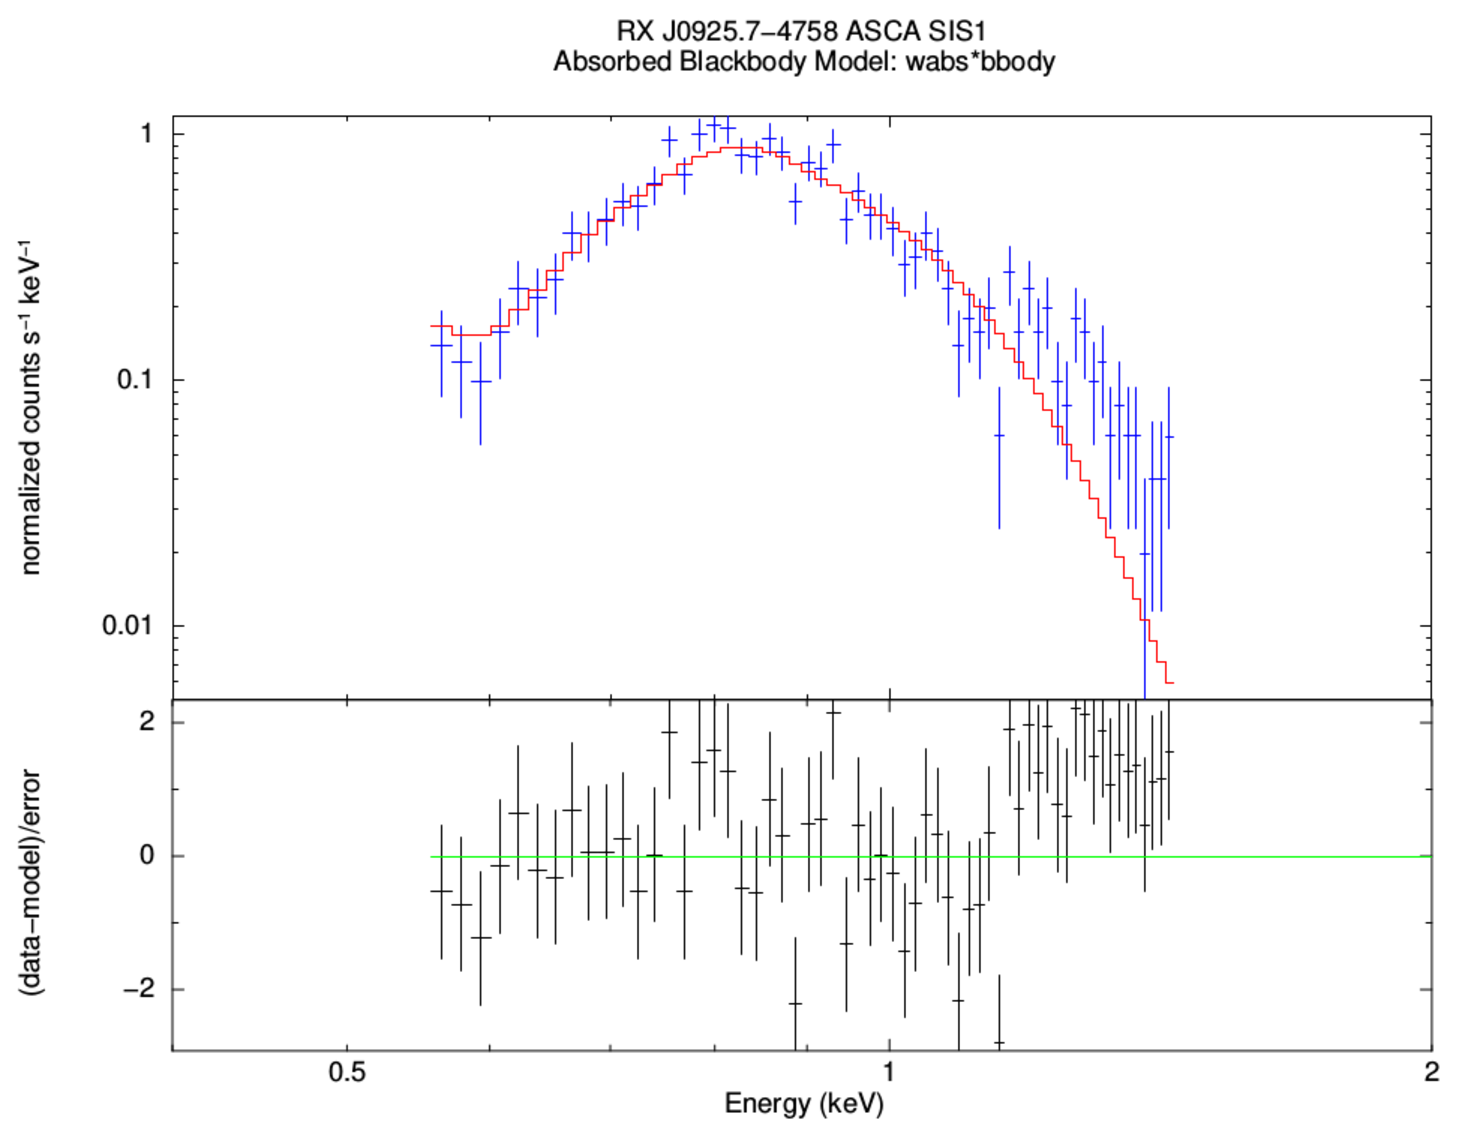
\includegraphics[scale=0.34]{mr-vel-asca-01.pdf}} %\hfill
					\subfloat[\texttt{ismabs*bbody} \label{asca:02}] {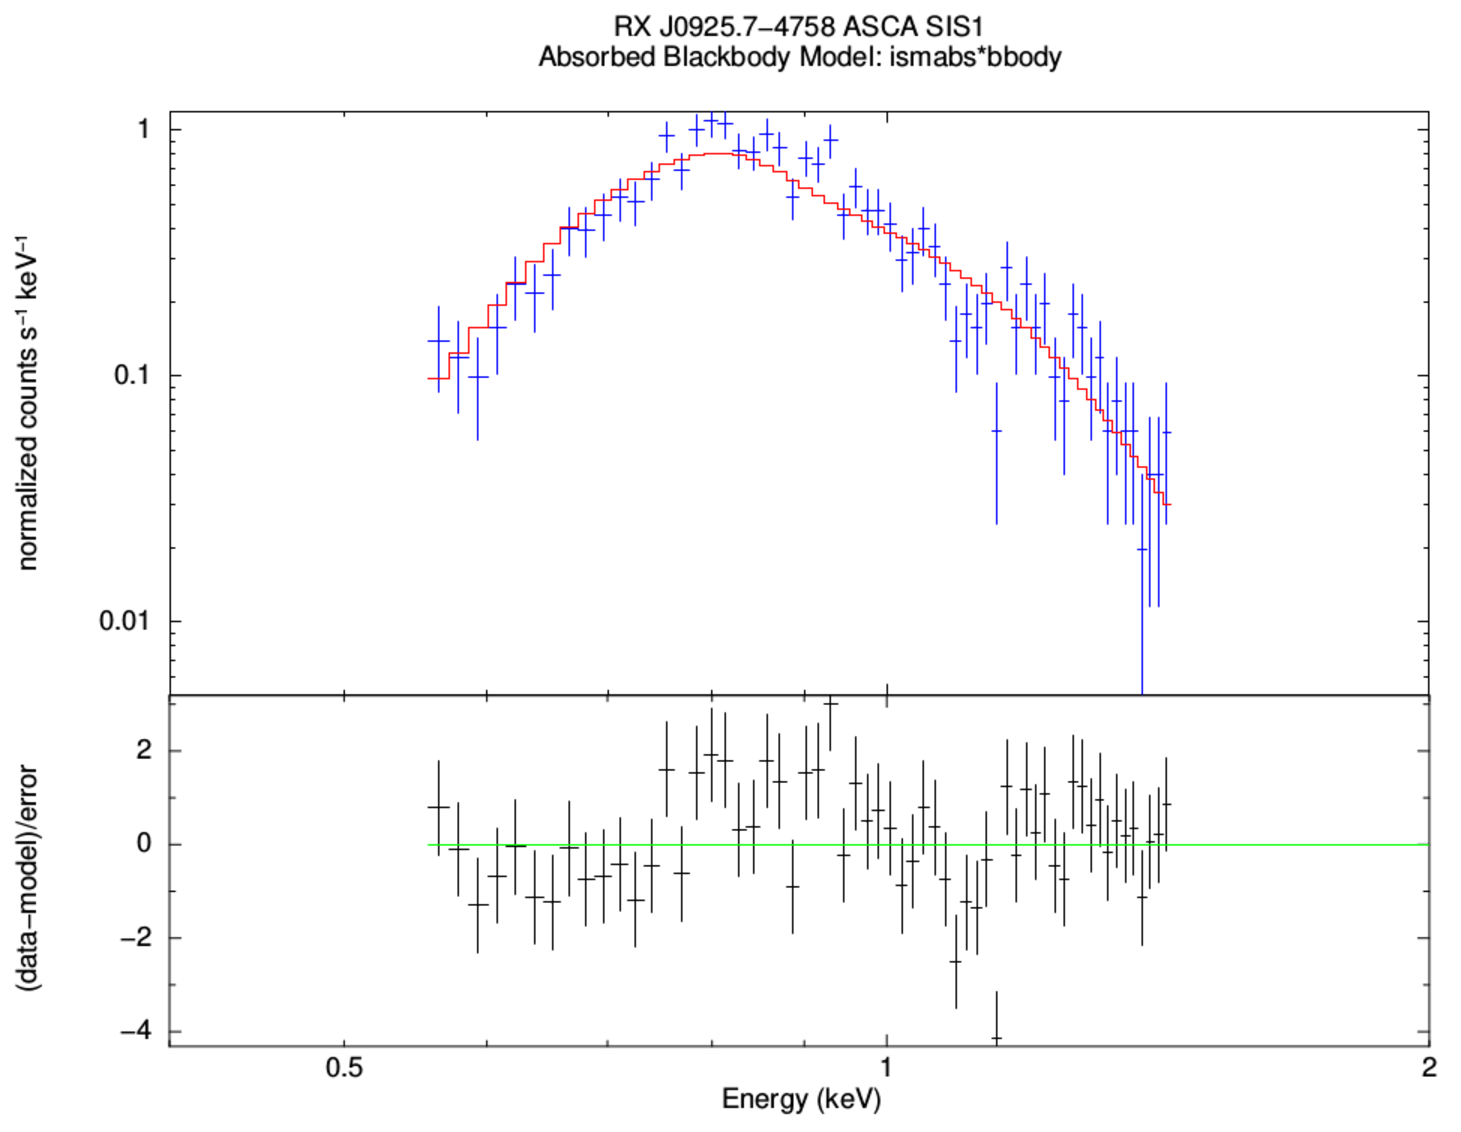
\includegraphics[scale=0.34]{mr-vel-asca-02.pdf}} %\hfill
				\end{figure}
				
				Table \ref{tab-asca:01} summarises the parameters obtained from fitting using an absorbed blackbody model.

				\begin{table}[h!]
					\begin{center}
						\caption{Spectral parameters from absorbed blackbody fit}
						\label{tab-asca:01}
						\begin{tabulary}{\textwidth}{CCC|C}
							\hline
							{Parameter} & {\texttt{wabs*bbody}} & {\texttt{ismabs*bbody}} & {Ebisawa \emph{et al.}} \\
							\hline
							{Temperature} & {50.0 eV} & {93.9 eV} & {46 eV} \\
							{$N_H$} & {$1.71\times 10^{22}$} & {$7.51\times 10^{21}$} & {$2.1\times 10^{22}$} \\
							{$L$ (0.4--2.0 keV)} & {$2.71\times 10^{36}$ erg/s} & {$2.96\times 10^{36}$ erg/s} & {$1.5\times 10^{36}$ erg/s} \\
							{$\chi_{\mathrm{reduced}}^2$} & {1.52} & {1.48} & {10.0} \\
							\hline
						\end{tabulary}	
					\end{center}
				\end{table}

			\subsection{Fitting using an Absorbed Blackbody with Absorption Edges} \label{continuum:asca:abs-bb-edge}
				The low-resolution spectrum gathered by ASCA indicates the presence of at least three absorption edges. At the next stage, we included three such edges in Xspec using the multiplicative model \texttt{edge}. This was done for both interstellar absorption components. In the \texttt{edge} model components, we have used the same values as mentioned by Ebisawa \emph{et al.}, i.e. at 0.94 keV, 1.04 keV and 1.43 keV.
				
				Figure \ref{asca:03} shows the spectrum fitted using an absorbed blackbody with edges model, with \texttt{Wabs} used to approximate the interstellar absorption. On the other hand, figure \ref{asca:04} illustrates the same model, but using \texttt{ISMabs}.
				
				\begin{figure}[h!]
					\centering
					\caption{Fitted ASCA spectrum using absorbed blackbody with edges model}
					\label{asca:abs-bb-edge}
					\subfloat[\texttt{wabs*edge*edge*edge*bbody} \label{asca:03}]{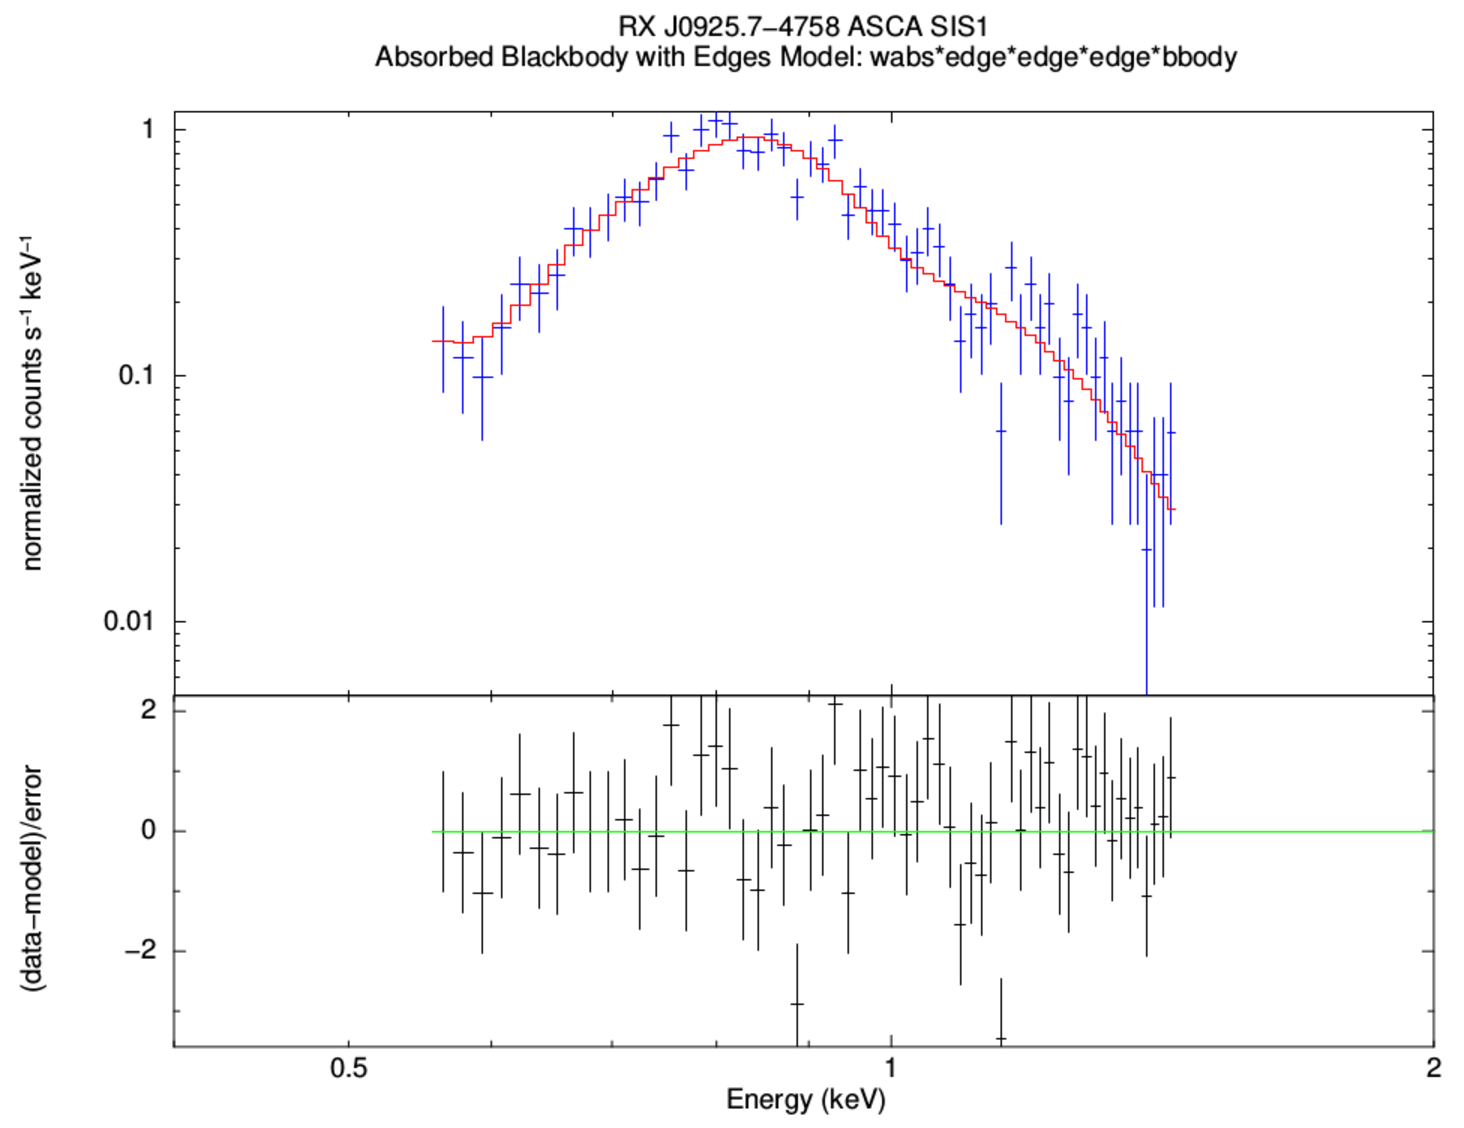
\includegraphics[scale=0.34]{mr-vel-asca-03.pdf}} %\hfill
					\subfloat[\texttt{ismabs*edge*edge*edge*bbody} \label{asca:04}] {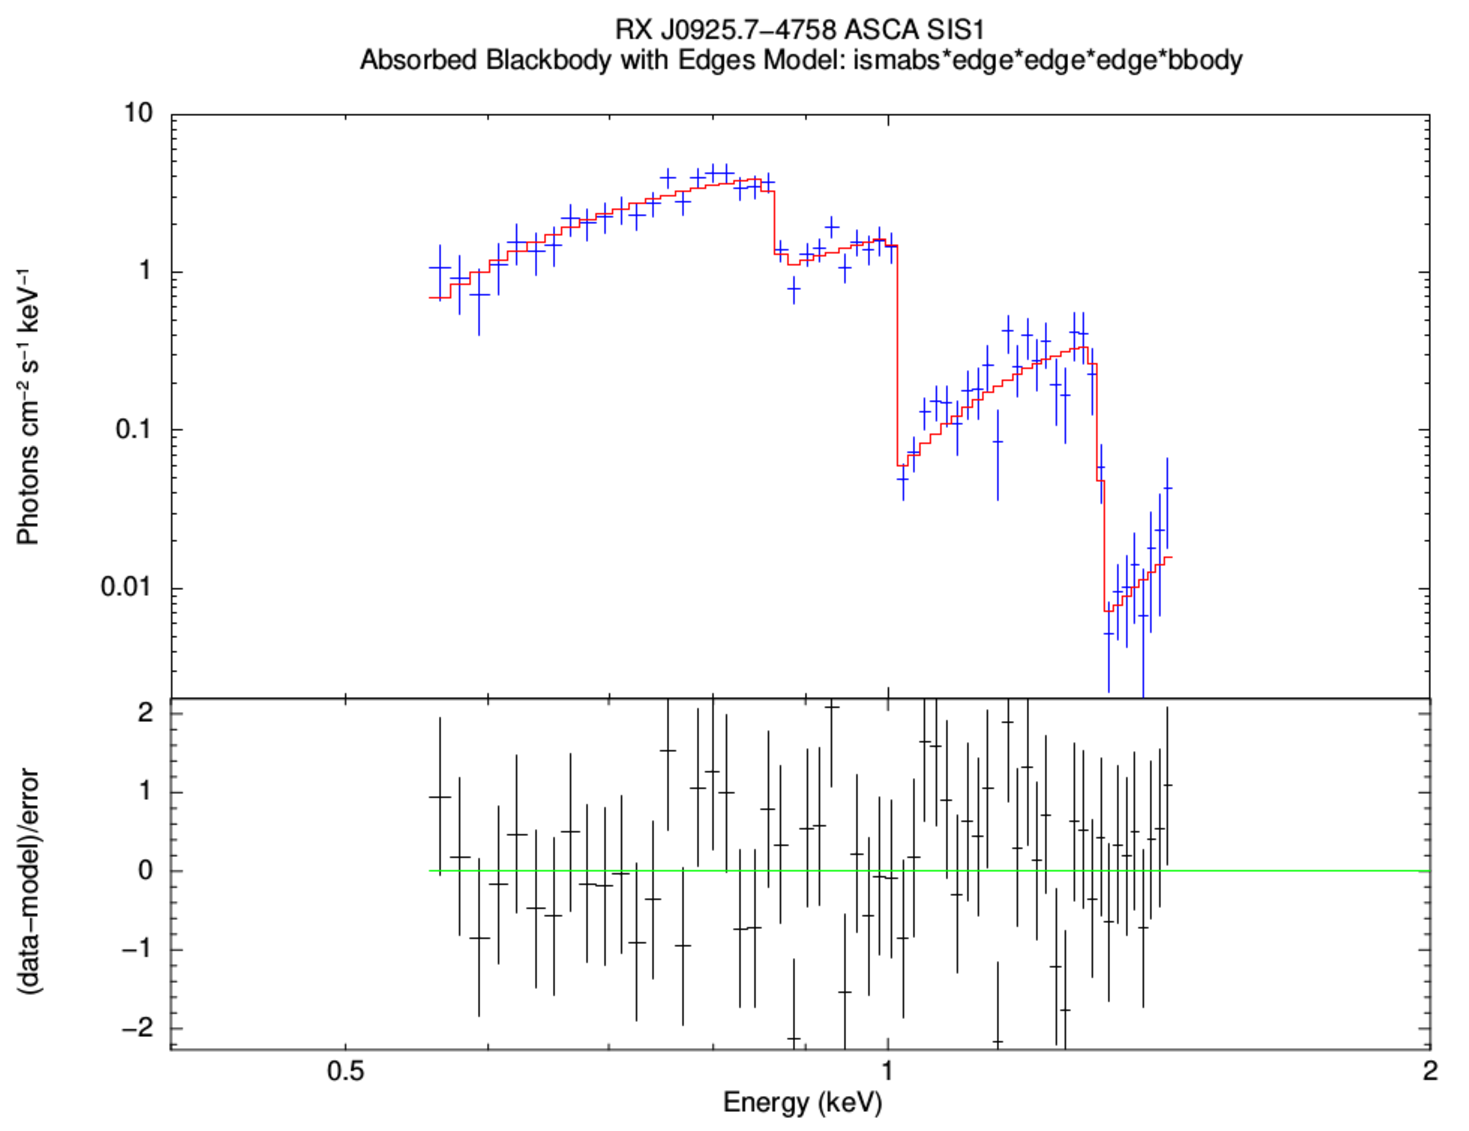
\includegraphics[scale=0.34]{mr-vel-asca-04.pdf}} %\hfill
				\end{figure}
				
				Table \ref{tab-asca:02} summarises the same when absorption edges are also included in the model, and includes the maximum optical depths obtained.
				
				\begin{table}[h!]
					\begin{center}
						\caption{Spectral parameters from absorbed blackbody with edges fit}
						\label{tab-asca:02}
						\begin{tabulary}{\textwidth}{CCC|C}
							\hline
							{Parameter} & {\texttt{wabs*edge$^3$*bbody}} & {\texttt{ismabs*edge$^3$*bbody}} & {Ebisawa \emph{et al.}} \\
							\hline
							{Temperature} & {83.9 eV} & {124.0 eV} & {96 eV} \\
							{$N_H$} & {$1.02\times 10^{22}$} & {$2.15\times 10^{22}$} & {$1.0\times 10^{22}$} \\
							{$L$ (0.4--2.0 keV)} erg/s & {$2.88\times 10^{36}$} & {$3.08\times 10^{36}$} & {$2.10\times 10^{36}$} \\
							{$\tau_{\mathrm{max}}$ for 0.94 keV edge} & {$1.41$} & {$0.54$} & {$0.65$} \\
							{$\tau_{\mathrm{max}}$ for 1.04 keV edge} & {$1.8\times 10^{-8}$} & {$3.20$} & {$1.19$} \\
							{$\tau_{\mathrm{max}}$ for 1.43 keV edge} & {$1.5\times 10^{-8}$} & {$2.2\times 10^{-8}$} & {$1.20$} \\
							{$\chi_{\mathrm{reduced}}^2$} & {1.21} & {1.01} & {1.02} \\
							\hline
						\end{tabulary}	
					\end{center}
				\end{table}
		
		\section{Fitting of XMM-Newton EPIC-pn Data} \label{continuum:xmm-epic}
			As evident from tables \ref{tab-asca:01} and \ref{tab-asca:02}, the \texttt{ISMabs} component seems to give a better fit. Also, the presence of absorption edges seem to improve the fit. Therefore, we have retained \texttt{ismabs} and \texttt{edge}, along with \texttt{bbody} in our basic continuum model. Then onwards, we proceeded to add other model components in an attempt to obtain a better fit with spectra of higher resolution, namely the spectra gathered by the EPIC-PN and RGS.
			
			\subsection{With EPIC-pn Data} \label{continuum:xmm-epic:pn}
				The model, which was applied to obtain figure \ref{asca:04}, was applied as is on the PN spectrum. The resulting fit was unacceptable, with a reduced $\chi^2$ of 25.4.
				
				\begin{figure}[h!]
					\centering
					\caption{Fitted XMM spectrum using absorbed blackbody with edges model}
					\label{xmm:abs-bb-edge}
					\subfloat[\texttt{ismabs*edge*edge*edge*bbody} \label{xmm-pn:01}]{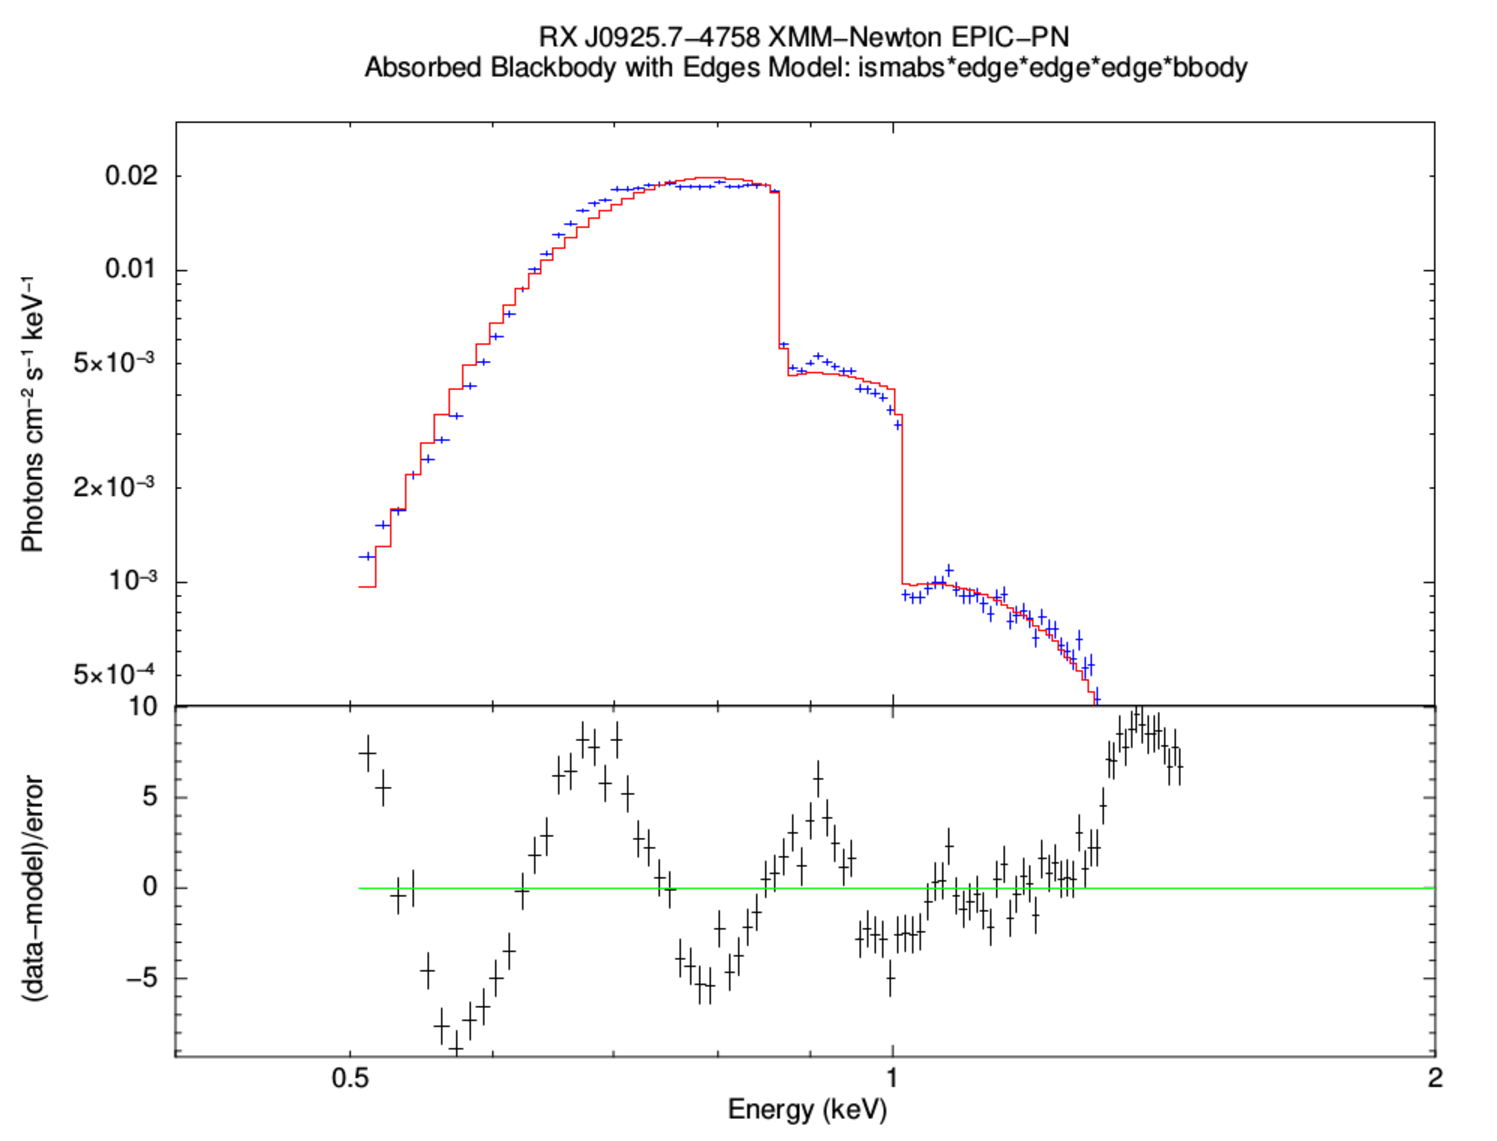
\includegraphics[scale=0.34]{mr-vel-xmm-pn-01.pdf}} %\hfill
				\end{figure}
				
				As can be seen from figure \ref{xmm-pn:01}, there is a significant oscillation between data and model, mainly for the soft X-ray photons. To remedy this, another additive model component, namely \texttt{gaussian}, was combined with the existing \texttt{bbody} component to give the following composite model:
				\begin{center}
					\texttt{ismabs*edge*edge*edge*(gaussian+bbody)}
				\end{center}
				
				
				\begin{figure}[h!]
					\centering
					\caption{Fitted XMM spectrum using composite model}
					\label{xmm:composite}
					\subfloat[\texttt{ismabs*edge*edge*edge*(gaussian+bbody)} \label{xmm-pn:01}]{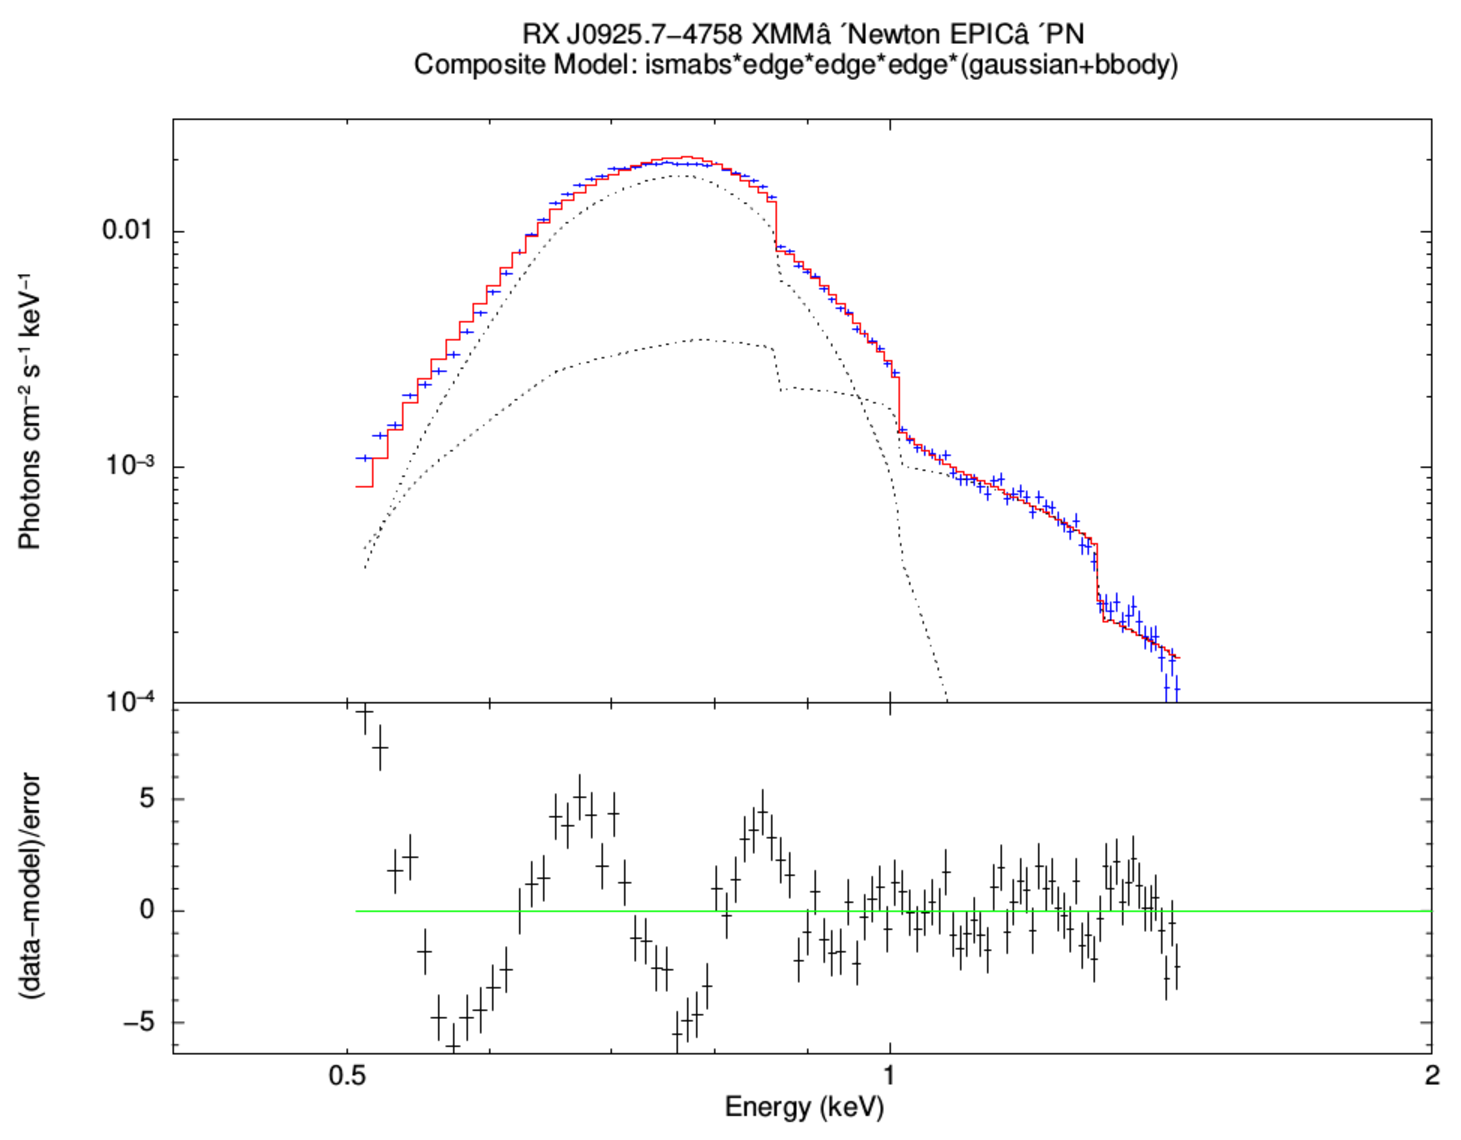
\includegraphics[scale=0.34]{mr-vel-xmm-pn-02.pdf}} %\hfill
				\end{figure}
				
				From figure \ref{xmm:composite}, it can be seen that the difference between data and model has reduced for the hard photons, even though there has been only marginal improvement in case of softer photons. Perhaps this is also reflected in the improvement in the reduced $\chi^2$, as compared to the previous model.
				
				A reduced $\chi^2$ of 8.31 was obtained at the end of the fitting. Also, among the metals, the \texttt{ISMabs} seems to show significant abundances for NeI, MgI and ArI, at $1.12\times 10^{18}$, $3.18\times 10^{18}$ and $6.62\times 10^{15}$ respectively, as compared to the other metals included in the model.
